\subsubsection{06.01.2016}
\textit{\textbf{Time frame:}} 17:00-21:30 \newline
Today it was created the working version of a device for preventing the bending of slats for shifting the bucket. It was tested and it was accepted that the device worked ok.
The chain at the winch was installed.
The elevator was tested. Firstly, it was found out, that one pair of blocks is fixed not reliable enough. The problem was that due to the cable was not in a plane of the block, it was pulled up by the cable. To compensate this pressure there were installed two plastoc clamps. However, it was a temporary solution.

Secondly, the power of 3 motors still was not enough to extract the elevator to the full. The problem was that the second sectoin (with respect to the bottom) required more power for extraction than the first one and the third section required the most power. So, it was assumed, that the problem caused by overloading the friction of the blocks: in the current system one cable at each side was held through all the blocks and a large part of power was wasted on friction. In this case, to reduce the power that spends on foghtin the friction, it was decided to use another system of helding the cables. The new construction required 3 blocks instead of 5 at a side and the cable from the winch went only through one of them. However, this construction required three times higher torque and three times less length of the cable to reel for extracting. So, the diameter of the coils chould be changed correcpondingly.

Today it was also continued the development or the mechanism for scoring autonomus alpinists. It was created a mechanism for releasing the climbers.

\begin{figure}[H]
	\begin{minipage}[h]{1\linewidth}
		\center{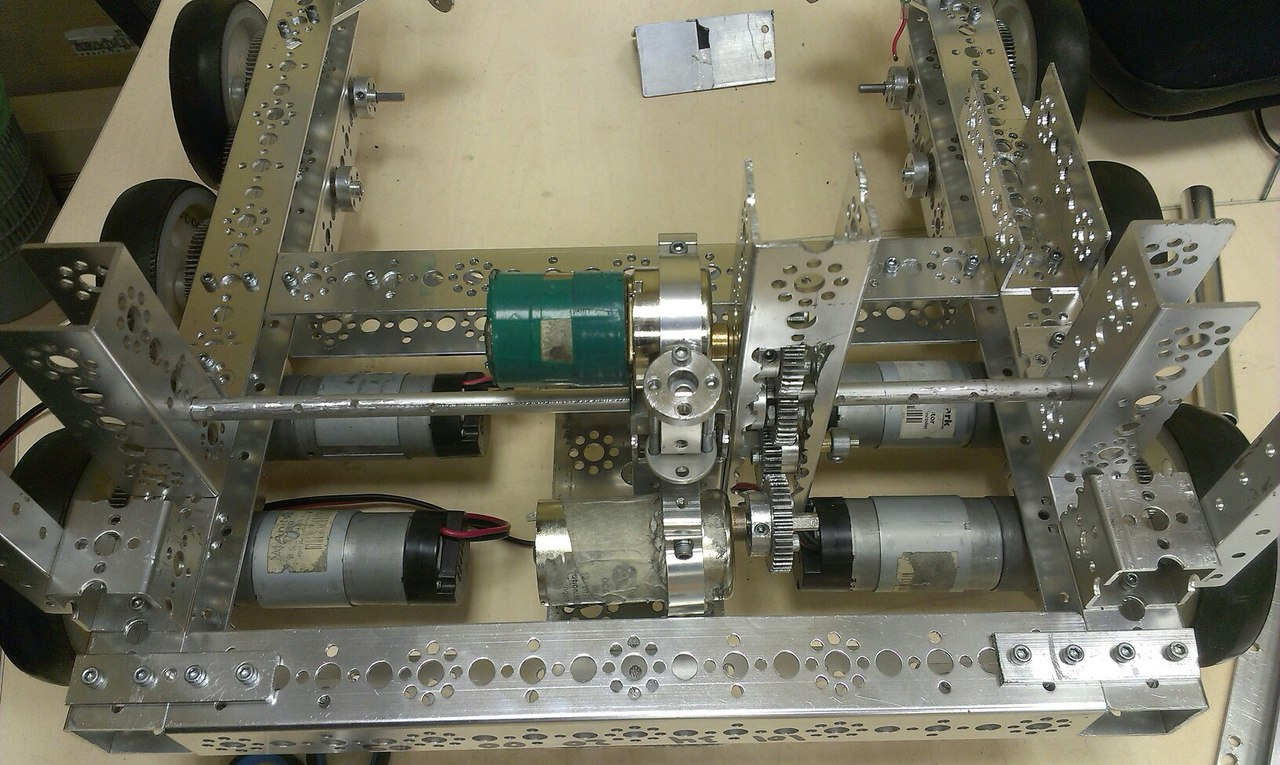
\includegraphics[scale=0.2]{3Engineering/5Team_meetings/days_of_meetings/2015.12.17/images/01}}
		\caption{Wheel base with 10cm wheels}
		\label{wheeel_base_10cm_wheels}
	\end{minipage}
\end{figure}

